\documentclass[a4paper,12pt]{article}

\usepackage{graphicx}
\graphicspath{{figures/}}
\usepackage{geometry}
\geometry{
    a4paper,
    total={170mm,257mm},
    left=20mm,
    top=20mm,
    }
\geometry{textwidth=426pt}
\usepackage{tabularx, ragged2e}
\usepackage{mathtools}
\usepackage{multicol}
\usepackage{titlesec}

\titleformat{\section}{\fontsize{11}{15}\bfseries}{\Roman{section}}{1em}{}
\titleformat{\paragraph}{\normalfont}{\textbf{\theparagraph.}}{0.5em}{}
\titlespacing*{\paragraph}{1.5em}{0.5em}{0.5em}
\counterwithout{paragraph}{section}
\setcounter{secnumdepth}{4}


\begin{document}

%\scshape
\centering
\onecolumn

\noindent
\begin{minipage}[]{0.7\textwidth}
\large{Practicum 1 $-$ group A \\Enzymatic activity of nitrophenyl-phosphatase}\par \vspace{0.1em}
\footnotesize{Quantitative cell analysis \& tissue engineering}\vspace{0.6em}
\flushleft
\begin{tabularx}{\widthof{\large{MAKING TITLES IN \LaTeX}}}{X l}
Team:  & Céline Duchaine\\
& Leen van Kerckhoven \\
& Lucas Comyn \\
& Vincent Belpaire \\
%Role: & Student at USI\\
%Supervisor: & Julien Prokofiev\\
Date: & October 5, 2022
\end{tabularx}


\end{minipage}% PUT THIS HERE!
\begin{minipage}[]{0.3\textwidth}
\flushright{

\includegraphics[width=3cm, keepaspectratio]{logo_ghent.png} \par \vspace{0.1cm}
\texttt{Faculty of engineering and architecture}
}
\end{minipage}

\flushleft

\section{Standard curve for nitrophenol}

\paragraph{Make a plot of the absorbance versus concentration and calculate the trendline. ($E=bx+a$ with $x=$ nitrophenol concetration) And calculate the concentration of P01.}

\begin{figure}[htb]
    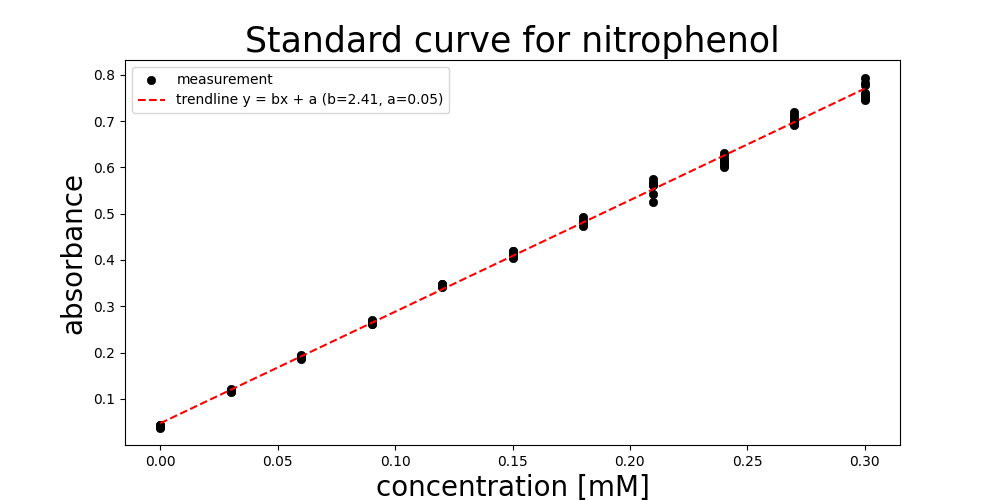
\includegraphics[scale=0.4]{fig1.png}
    \centering
\end{figure}

The estimated concentration of PO1 is 0.01743 mM. (We made the mean of all of the results to estimate it's concentration.)

\section{Enzymatic activity as a function of substrate concentration}

\paragraph{Plot the enzymatic activity (as absorbance after 30 minutes (Y-axis)) 
against the substrate concentration (X-axis) and display $R^2$.}

Note: in this expirement the absorbance was measured after 20 minutes.

\begin{figure}[htb]
    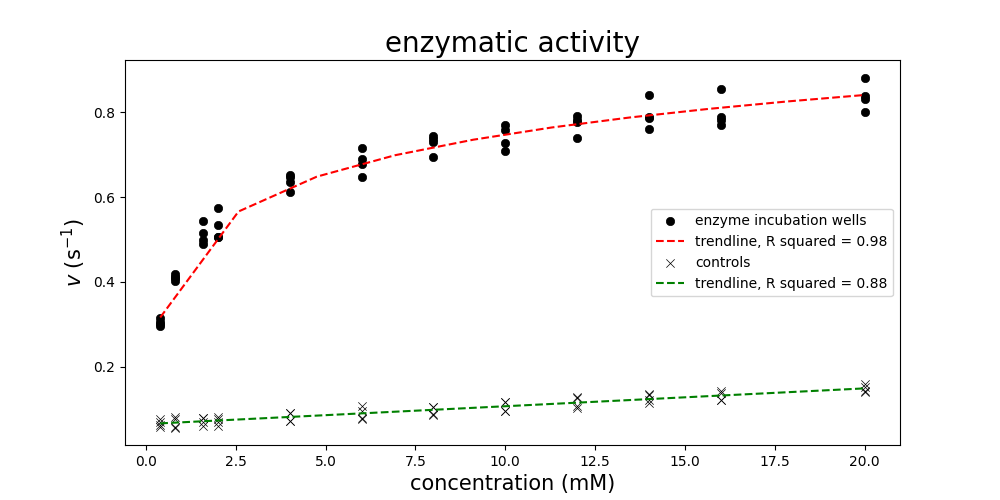
\includegraphics[scale=0.4]{fig2_1.png}
    \centering
\end{figure}

$v$ (enzymatic activity) is calculated as $\frac{\text{absorbance}}{1200 \text{s}}$, 1200 s = 20 min in oven, with absorbance a dimensionless quantity, hence $v$ got untis $\frac{1}{\text{s}}$.\\

\paragraph{Lineweaver-Burk plot: $\frac{1}{v}$ (Y-axis) against $\frac{1}{[S]}$ (X-axis) and display $R^2$. 
Formula of Michaëlis Menten:\[v=V_{\text{max}}\frac{[S]}{K_m+[S]}\] \[\frac{1}{v}=\frac{1}{V_{\text{max}}}\left(\frac{K_m}{[S]}+1\right)\]}

\begin{figure}[htb]
    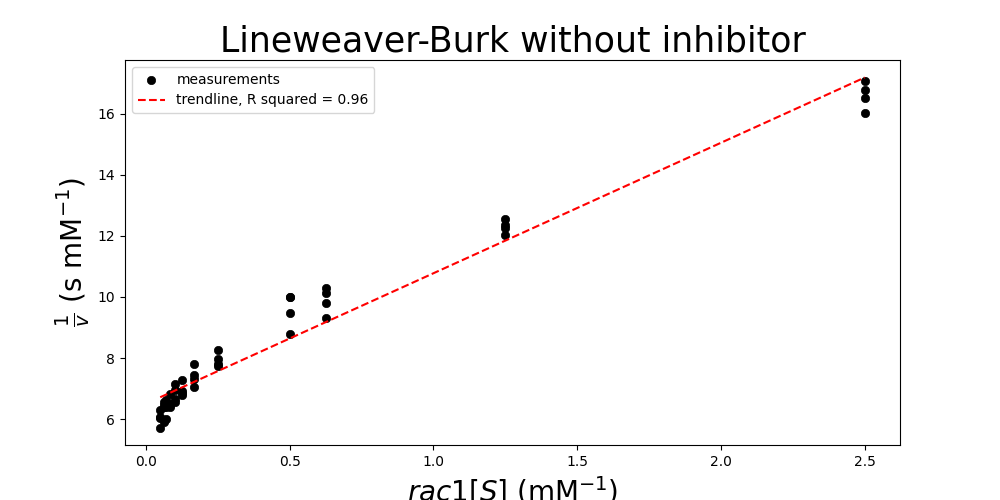
\includegraphics[scale=0.4]{fig2_2.png}
    \centering
\end{figure}

\paragraph{Eadie-Hofstee plot: $\frac{v}{[S]}$ (X-axis) against $v$ (Y-axis) and display $R^2$. \[v=-K_m\frac{v}{[S]}+V_{\text{max}}\]}

\begin{figure}[htb]
    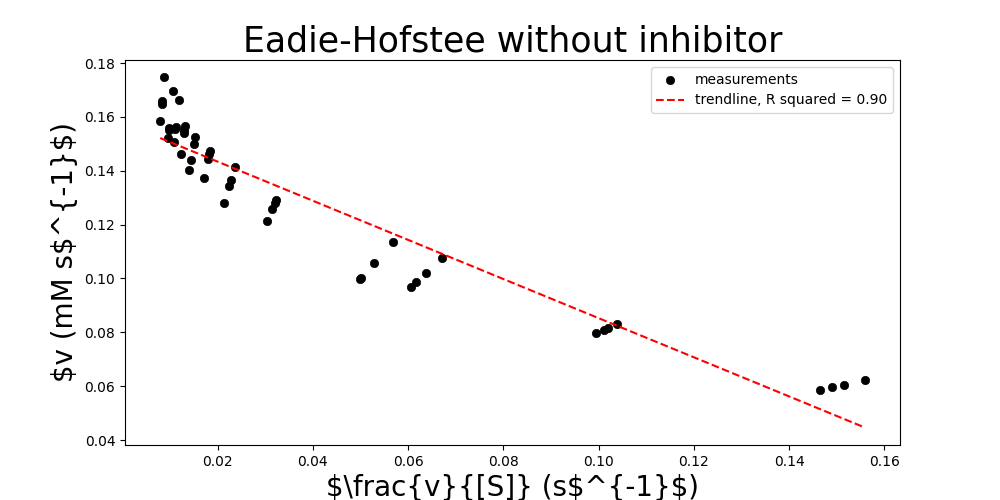
\includegraphics[scale=0.4]{fig2_3.png}
    \centering
\end{figure}

\paragraph{Hanes-Woolf plot: $\frac{[S]}{v}$ (Y-axis) against $[S]$ (X-axis) and display $R^2$. \[\frac{[S]}{v}=\frac{[S]}{V_{\text{max}}}+\frac{K_m}{V_{\text{max}}}\]}

\begin{figure}[htb]
    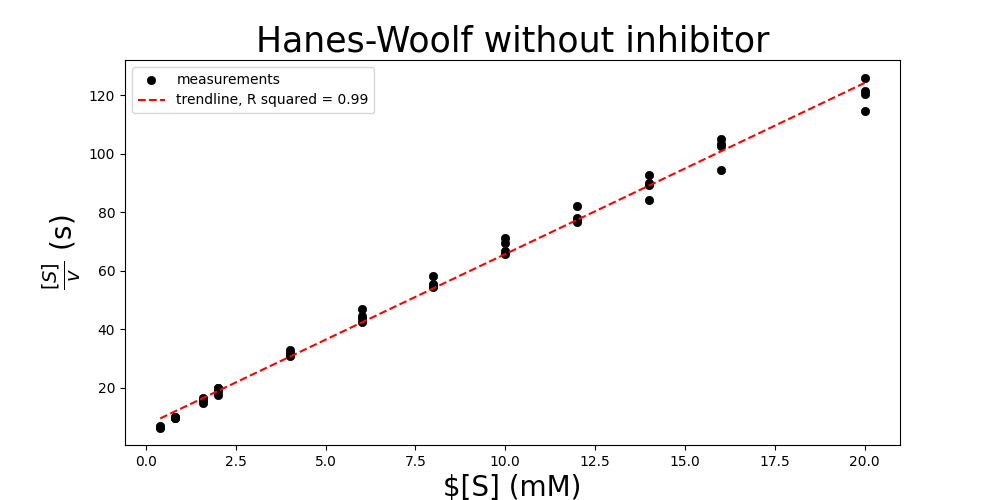
\includegraphics[scale=0.4]{fig2_4.png}
    \centering
\end{figure}

\paragraph{Calculate $K_m$-values (molarity of substrate in incubation mixture) and $V_{\text{max}}$ (formed nitrophenol (mg) per 30 minutes) for every plot. Do you observe 
differences? Why?}

The $K_m$ and $V_{\text{max}}$ value can be derived from the trendline ($y = bx+a$):
\begin{itemize}
\item Lineweaver-Burk plot: $V_{\text{max}} = \frac{1}{a} = 0.15\: \frac{1}{\text{s}}$, $K_m = \frac{b}{a} = 0.66$ mM
\item Eadie-Hofstee plot: $V_{\text{max}} = a = 0.16\: \frac{1}{\text{s}}$, $K_m = -b = 0.73$ mM
\item Hanes-Woolf plot: $V_{\text{max}} = \frac{1}{b} = 0.17\: \frac{1}{\text{s}}$, $K_m = \frac{a}{b} = 1.22$ mM
\end{itemize}

\section{Enzymatic activity in the presence of an inhibitor}

\paragraph{Plot the enzymatic activity (as absorbance after 30 minutes (Y-axis)) 
against the substrate concentration (X-axis). Add a trendline and $R^2$}

Note: in this expirement the absorbance was measured after 20 minutes.

\begin{figure}[htb]
    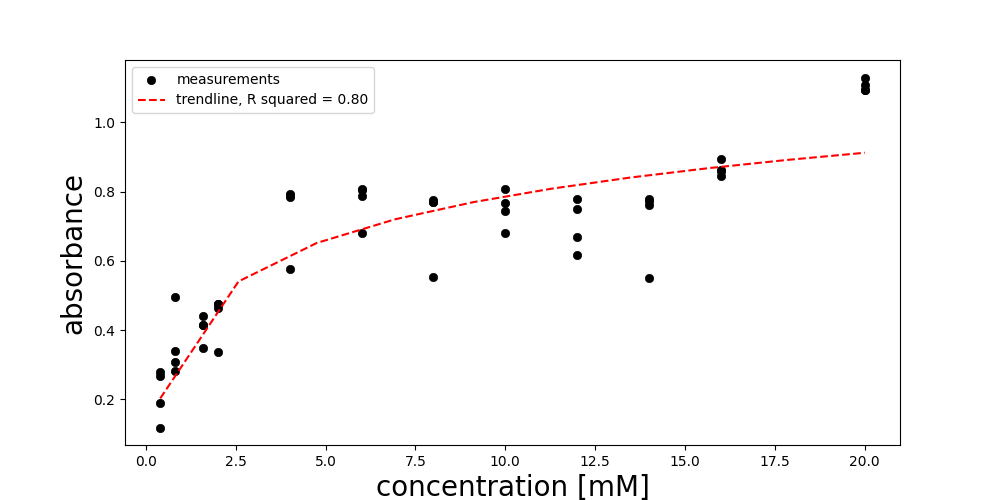
\includegraphics[scale=0.4]{fig3_1.png}
    \centering
\end{figure}

$v$ (enzymatic activity) is calculated as $\frac{\text{absorbance}}{1200 \text{s}}$, 1200 s = 20 min in oven, with absorbance a dimensionless quantity, hence $v$ got untis $\frac{1}{\text{s}}$.\\

\paragraph{Lineweaver-Burk plot: $\frac{1}{v}$ (Y-axis) against $\frac{1}{[S]}$ (X-axis).}

\begin{figure}[htb]
    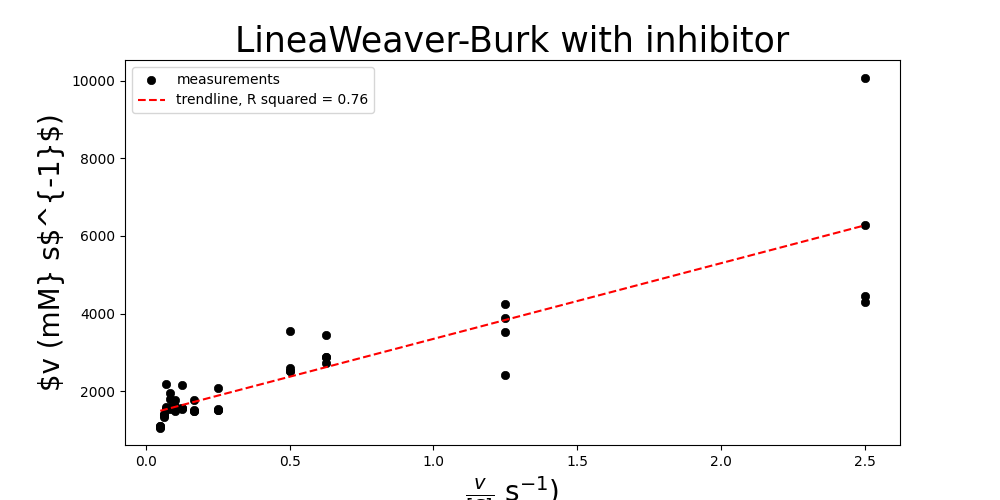
\includegraphics[scale=0.4]{fig3_2.png}
    \centering
\end{figure}

\paragraph{Eadie-Hofstee plot: $\frac{v}{[S]}$ (X-axis) against $v$ (Y-axis).}

\begin{figure}[htb]
    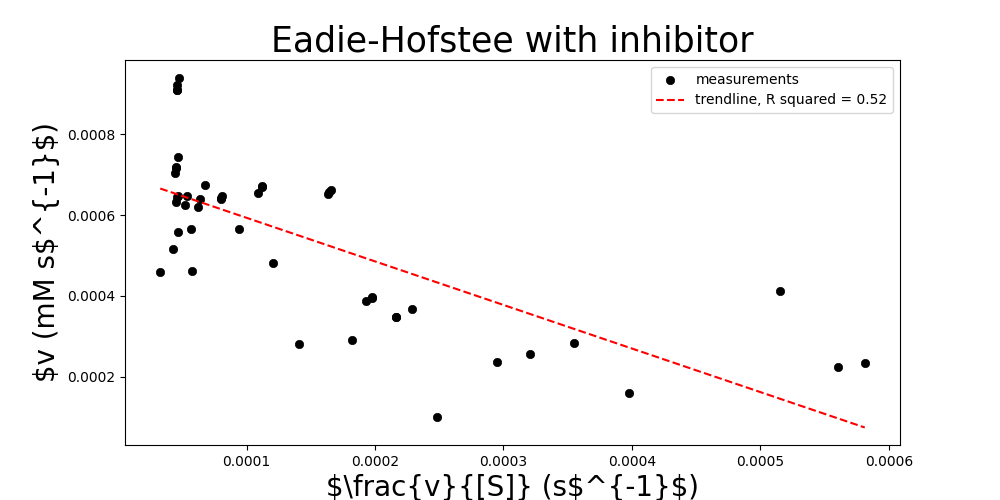
\includegraphics[scale=0.4]{fig3_3.png}
    \centering
\end{figure}

\paragraph{Hanes-Woolf plot: $\frac{[S]}{v}$ (Y-axis) against $[S]$ (X-axis).}

\begin{figure}[htb]
    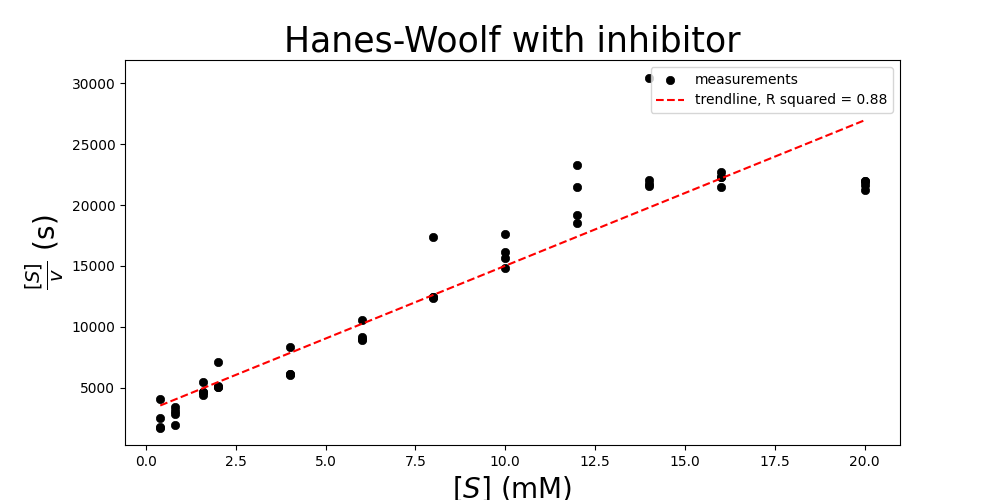
\includegraphics[scale=0.4]{fig3_4.png}
    \centering
\end{figure}

\paragraph{Calculate $K_m$-value (molarity of substrate in incubation mixture) and $V_{\text{max}}$ (formed nitrophenol (mg) per 30 minutes) for every plot.}

The $K_m$ and $V_{\text{max}}$ values can be derived from the trendline ($y = bx+a$):
\begin{itemize}
\item Lineweaver-Burk plot: $V_{\text{max}} = \frac{1}{a} = 0.000716\: \frac{1}{\text{s}}$, $K_m = \frac{b}{a} = 1.40$ mM
\item Eadie-Hofstee plot: $V_{\text{max}} = a = 0.000701\: \frac{1}{\text{s}}$, $K_m = -b = 1.08$ mM
\item Hanes-Woolf plot: $V_{\text{max}} = \frac{1}{b} = 0.000836\: \frac{1}{\text{s}}$, $K_m = \frac{a}{b} = 2.55$ mM
\end{itemize}

\paragraph{Is the inhibitor competitive or non-competitive? Motivate your answer.}

\begin{figure}[htb]
    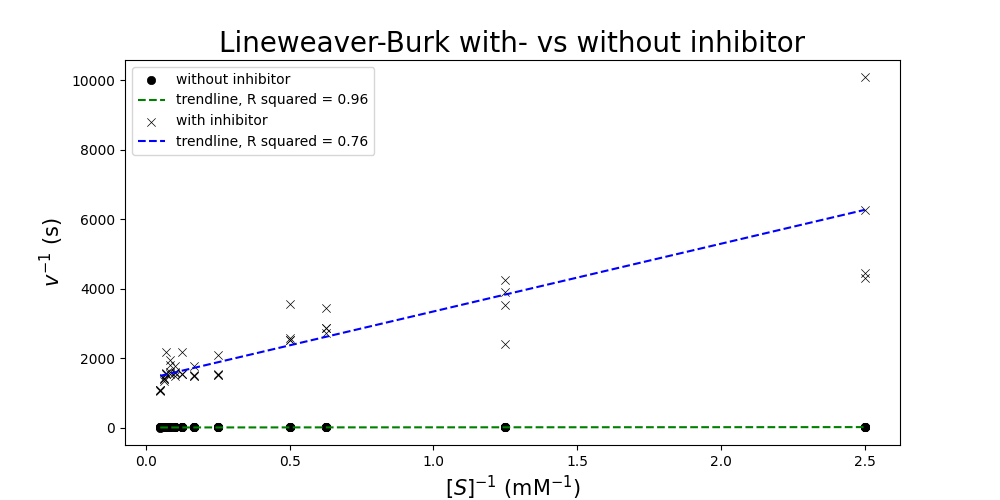
\includegraphics[scale=0.4]{fig3_6.png}
    \centering
\end{figure}

It is a non-competitive inhibitor: differrent $V_{\text{max}}$ and not parallel. (Remark: $\Delta V_{\text{max}} \gg \Delta K_m \Rightarrow$ assume "constant" $K_m$ values)

\end{document}
